The goal of this work is to understand which transformations are necessary to convert a program from a sequential programming model with shared memory into a distributed, concurrent programming model of a microkernel operating system. A significant part of these transformations is already implemented in the Ohua compiler. Therefore, the specific goal is to understand and close the 'translation gaps' between the programming models of the source program, the current Ohua implementation, and the M3 operating system. So to better understand the work that need to be done, we will introduce those models in this chapter.

\section{Ohua}
\label{sec:back_ohua}
In this section we will introduce the Ohua compiler\cite{ertel2015ohua}. Its essential concept is to extract the underlying data flow graph from a sequential input program. The result is a program structure consisting of individual steps that are connected only by incoming and outgoing data and can be executed concurrently. These individual steps and their data channels can then be mapped to various abstractions of processes and communication channels in the backend of the compiler to achieve parallelization and isolation of the steps. Like most compilers, Ohua works step-by-step with different intermediate representations (IRs) of the input program. To be able to support different languages and target architectures, Ohua uses language integrations. Currently there are integrations for Rust and Python. In the next subsection, we will take a closer look at the basic structure and function of Ohua. 

For this work, it is also important to understand what programming model Ohua currently supports. Here, programming model means on the one hand which restrictions in the syntax of the input programs are currently necessary to be able to convert them into correct concurrent programs. On the other hand it contains the explicit and implicit assumptions about the concrete implementations of 'processes' and 'channels'. So we will also look at these aspects in more detail in this section.

\subsection{Compiler Pipeline}
\label{subec:OhuaPipeline}
When we say 'Ohua compiles a program', we mean it compiles functions in the compile scope. In contrast to e.g. rustc or gcc Ohua does not compile the complete code of the program, but transforms only the functions e.g. within one or more Python modules specified in the call. We call these functions algorithms. In contrast to algorithms, functions and methods that are imported and used within algorithms are not compiled. They are completely opaque to the compiler. This also means that Ohua does not require any syntax constraint in these imported functions and methods. An overview of the compiler pipeline is shown in Figure~\ref{fig:ohua_fine}.  

In the \textbf{compiler frontend}, algorithms of the target language are first parsed and translated into Ohua's frontend language (Frontend IR). This translation is implemented in language specific frontend integrations. That is, for each language supported by Ohua, such a frontend integration must exist. This integration parses algorithms of the input language and translates them into the syntax of the frontend IR. For non-supported syntax constructs, currently for example \rust{break} statements in loops, the compilation terminates at this point. The currently supported subset of Rust can be found in the Appendix~\ref{sec:RustIntegration}.

\begin{figure}[H]
    \centering
    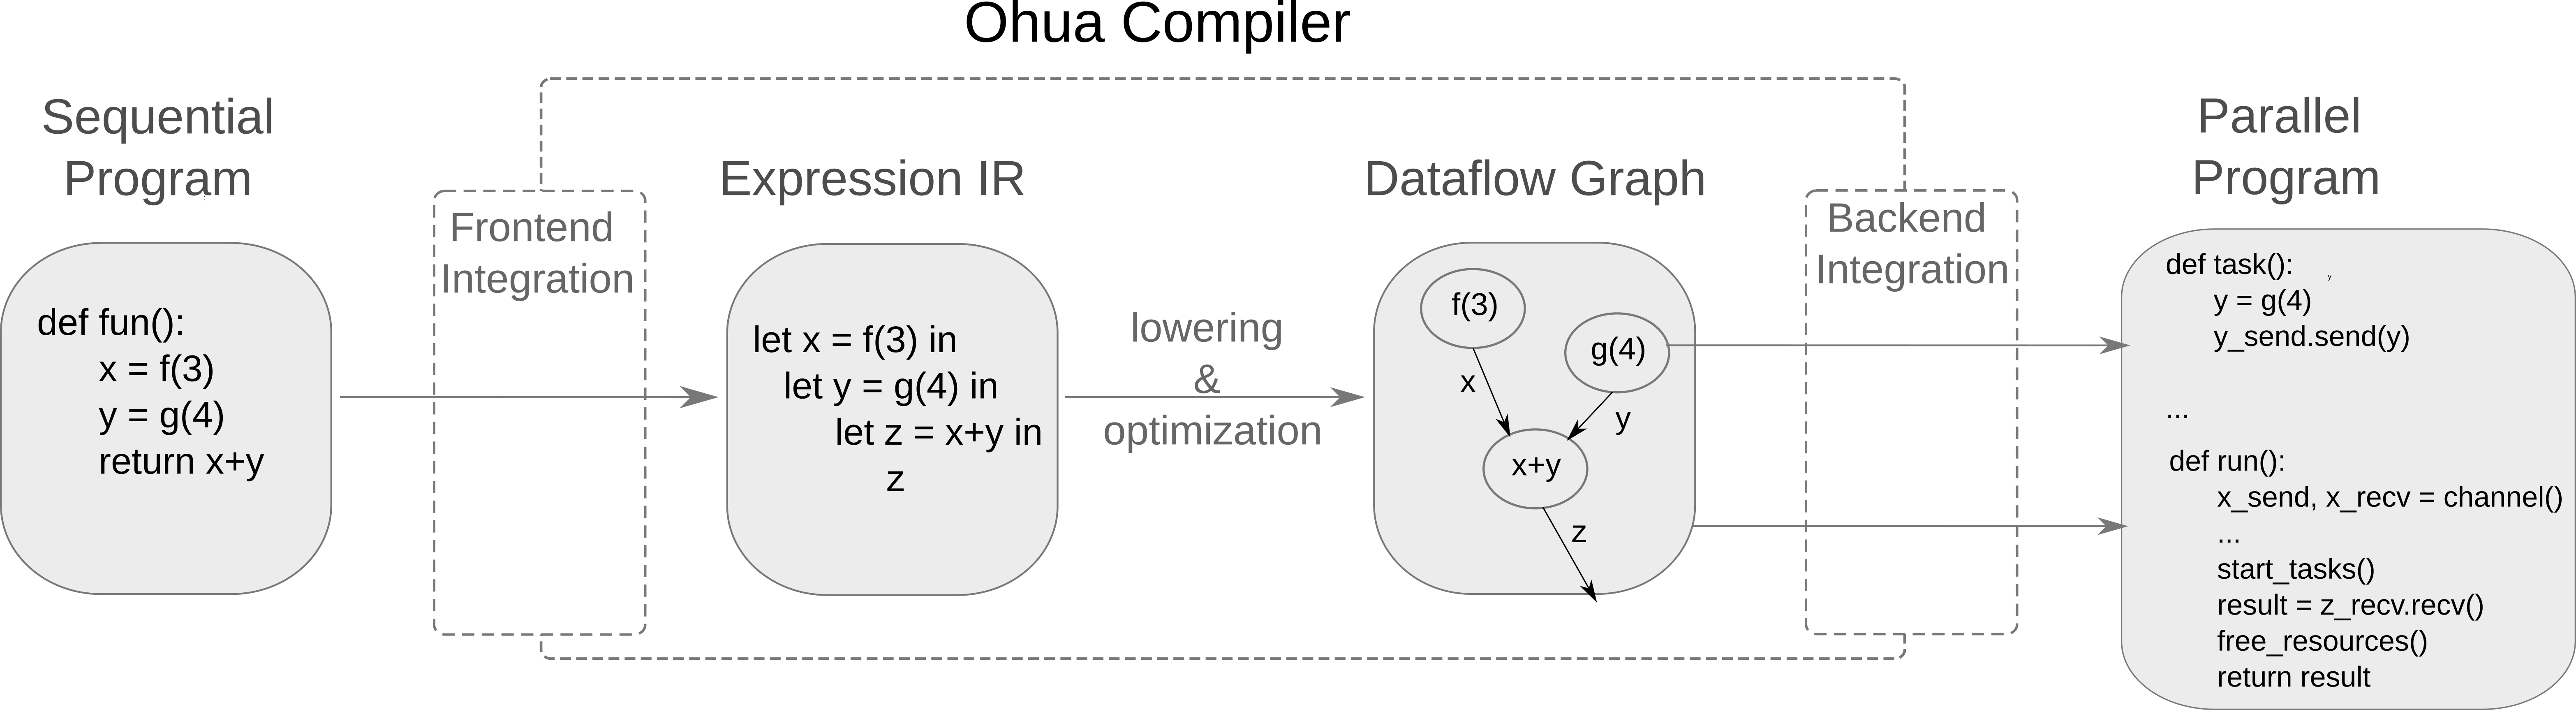
\includegraphics[scale= 0.36]{figures/ohua_fine_with_channels.png}
    \caption{Structural overview of Ohua and the code transformations}
    \label{fig:ohua_fine}
\end{figure}

In the \textbf{core compiler} itself there are two main representations of the code. One is Expression IR. This language is functional and based on the call-by-need lambda calculus. To transform input algorithms to this representation 
calls to other algorithms are inlined, renaming compiler passes ensure single static assignment form and assignment expressions are refactored to applicative normal form. A simplified example of code before and after the transformation is shown in Figure~\ref{fig:funBodyTranslation}. A central conversion step in the compiler is the transformation of stateful calls to so called \emph{state threads}(\cite{wadler1992essence}, \cite{launchbury1994lazy},\cite{ertel2019stclang}). To generate race condition free tasks, Ohua forbids shared state use and only permits stateful computation inside methods. However, methods in an imperative language mutate objects in place and implicitly refer to the new, changed state by the same reference as before. The conversion of stateful calls to state threads makes the semantic of creating a new state upon calling methods explicit. In the code example in Fig.\ref{fig:funBodyTranslation}, the call \rust{someState.do()}, is internally transformed to explicitly take a state as an argument and return a new, mutated state. Thereby, function calls downstream to not need to access a shared memory to use stateful objects. Based on this explicit state threading, Ertel et al. \cite{ertel2019stclang, ertel2018supporting} developed functional representations for imperative control flow on stateful computations. For example an imperative for-loop, is translated to a so called \rust{smap} operation, which is essentially a fold operation of the loop body on the states manipulated inside the loop. 

\begin{figure}
    \centering
    \begin{subfigure}[b]{0.45\textwidth}
         \centering
         \begin{minted}[fontsize=\small]{rust}
 fn algo(i){
   let someState = 
           other_algo(i);
   let a = someState.do()
   let b = f(a)
   return b
 }

 fn other_algo(i){
    let s = State::new(i)
    s
 }
            \end{minted}
         \caption{Input algorithm}
         \label{simplPyInput}
     \end{subfigure}
     \hfill
     \begin{subfigure}[b]{0.5\textwidth}
         \centering
         \begin{minted}[fontsize=\small, escapeinside=||,mathescape=true]{haskell}
let someState = 
        |$\lambda$| State::new (i) in
  let a, someState_0 = 
           |$\lambda$| do (someState, a) in
    let b = |$\lambda$| f (a) in
        b
        \end{minted}
        \vspace{15mm}
    \caption{Pseudocode of IR}
         \label{simplIR}
    \end{subfigure}
\caption{An algorithm is mapped to a nested let-expression with the innermost term representing its return value}
\label{fig:funBodyTranslation}
\end{figure}

The next representation in the compile flow is the Data Flow Graph (DFG) representation. Independent program tasks are encapsulated in the this representation and are explicitly assigned their incoming outgoing data channels. Besides function calls from the original program, this representation also contains control nodes that govern the data flow. For example if the input code contained a branching statement like \rust{if cond {f()} else {g()}} control nodes will be introduced to a) switch data flow between calls to \rust{f()} or \rust{g()} and b) to collect results from appropriate output channels of \rust{f()} or \rust{g()} depending on the condition. This representation also allows to merge certain nodes by fusing their code, as well as input and output channels. This is done for instance if a following node entirely depends on its predecessor and has so little work to do, that it would hardly justify the overhead of spinning up an independent task in any backend implementation.\\

Which ultimately brings us to the \textbf{compiler backend} and backend integrations of Ohua. Backend integrations consist of two parts. The 'Language Backend' is only language specific. Similar to the frontend integration, it serves the purpose of translating code inside tasks from Ohua representation syntax back to the target language syntax. The 'Architecture Backend' is responsible for translating the 'nodes' and 'edges' of the DFG into a specific implementation for concurrent tasks, communication channels and a runtime for the graph. For example their can be two different architectures for a given language one implementing tasks as threads, one using processes both also generating appropriate channels and runtime code to execute the DFG. As we did not compile imported functions the target language must match the input language, which is automatically ensured by the compiler. Architectures for the same language can be used interchangeably. This way Ohua can generate e.g. multi-threaded shared memory or fully distributed programs from the same input.\\

In the next section we will take a closer look at the restrictions and assumptions required to make this work.

\subsection{Programming Model}

The term programming model generally describes a relationship between syntax constructs in a programming language and their concrete semantics in a particular execution environment. In the case of Ohua, the programming model includes, on the one hand, the supported input syntax and the assumptions made about the supported terms of the input language. On the other hand, it specifies how these terms are translated into a dataflow graph and what assumptions Ohua makes about the implementation of nodes, edges, and runtime of the DFG. First we will look into the supported input syntax and assumed semantics. 

\subsubsection{Input Syntax and Semantics}
We already know, that Ohua's basic input unit are algorithms, i.e. pure functions inside the compile scope. Figure~\ref{tab:FrontendIR} depicts the language definition of the frontend representation described before. Any syntax construct of the input language has to be mapped to the according terms of these language to be compiled. In the following paragraphs we will describe the accepted syntax constructs and the semantics the programming model expects them to have. \\


\begin{table}[ht]
\resizebox{\columnwidth}{!}{%
    \begin{tabular}{l c l l}
        \multicolumn{4}{l}{\emph{Patterns:}}\\
        $p$ & $::=$ & $x\ |\ (x,~\ldots ,~x)\ |\ ()$ & named variables, tuples or unit\\
        \multicolumn{4}{l}{\emph{Expressions:}}\\
        $e$ & $::=$ & $e$ & named expression in host language\\
        & $|$ & $\textbf{1},\textbf{2},\textbf{3}, \ldots \ |\ \textbf{true}\ |\ \textbf{false}\ |\ \textbf{()} $ & typed literal in host language\\
        & $|$ & $\textbf{let}\ p\ \textbf{=}\ e\ \textbf{in}\  e$ & lexical scoping \\
        & $|$ & $e\ e$ & application\\
        & $|$ & $\boldsymbol{\lambda} [p,~\ldots ,~p]\textbf{.}\  e$ & abstraction \\
        & $|$ & $\textbf{if}\ e\ \textbf{then}\ e\ \textbf{else}\ e$ & conditionals\\
        & $|$ & $\textbf{map}\ e\ e$ & map first expression to second\\
        & $|$ & $\textbf{bind}\ e\ e$ & bind an expression representing a state to  \\
        & & & an expression representing a function to act on this state \\
        & $|$ & $\textbf{stmt}\ e\ e$ & expression whose return value is ignored\\
        & $|$ & $\textbf{seq}\ e\ e$ & \\
        & $|$ & $\textbf{(}\ e\ \textbf{)}$ & tuple of expressions \\
    \end{tabular}%
    }
    \caption{Definition of the Expression IR}
    \label{tab:FrontendIR}
\end{table}

\textbf{Function Calls:} Beside algorithms, Ohua supports stateful and stateless function calls, i.e. methods and pure functions, imported into the scope. Pure functions are expected to be side effect free. In particular the programming model assumes, that pure functions do not implicitly manipulate their arguments. This excludes for instance functions that manipulate their arguments by reference. If the output of a pure function call is not used it is considered to have no effect and is removed during compilation. 

Stateful function calls on the other hand are expected to manipulate the object they are called on, i.e. have a side effect. Consequently they are not removed regardless if the output is used. 
Any stateful computation is expected to happen exclusively and explicitly using  method calls and also method calls are expected to only manipulate the object state itself. This also entails the requirement, that state is not 'leaked' via return values. For example in the method call \rust{let x = SomeState.do_stuff();}, \rust{x} must not be, or contain a reference to \rust{SomeState}. We already assumed, that other functions do not manipulate \rust{SomeState} when using \rust{x} as argument. However without this 'leaking assumption' it would be possible to call \rust{x} as a stateful object, thereby implicitly manipulating the state of \rust{SomeState}. This implicit semantic is not handled currently and would be lost in the distributed output code. 

Functions need to be typed or type-able by the frontend integration. To correctly annotate the types in generated code, at least to the extend required for any particular backend and architecture, Ohua needs to extract type information from the input code. Specifically the argument types of each function call are extracted and preserved in the different IRs as typed function literals capturing the argument types of each function call. 

\textbf{Loops}: Ohua supports bound and unbound \rust{for}-loops. They are transformed into parallelizable pipelining of the independent calculation steps inside the loop. Inside for-loops each state from outside the loop must be used at most once to enable the accumulation of state changes in a single node for each object. Conditional loops (\rust{while} or \rust{do-while}) are as of the beginning of this work not supported, but can be expressed using recursion.

\textbf{Recursion}: Ohua supports recursion with some notable restrictions. Recursive algorithms must be tail recursive, the recursive call must be located in the if-branch, the return value must be in the else-branch of recursion. Further either one must be the only statement in each branch respectively. As return values only single variables are supported. Recursive loops will not yield any pipelining or parallelization but a loop executed for one input at a time. This is due to the semantic of recursion, being a repeated function on a state, where the result of each step depends not only on the step but also on previous results.
Currently the output of recursive algorithms can not be used in an assignment i.e. a recursive call can only be the last statement in another algorithm and return the calling algorithms final result. 

\textbf{Branching:} Branching is supported in case of simple if-else expressions, where both branches must be present. Also if-else statements as for instance present in the Python syntax are not supported currently. This is because in those statements have a different execution semantic than expressions i.e. branches that do not return a value but have side effects on variables from the surrounding scope. So they need to be implemented separately. Also it is currently not possible to use  stateful functions in branches.

\textbf{Return, Continue, Break:} Ohua does currently not support any forms of early return of conditional execution except for recursion and branching as described before. Therefor \rust{break} and \rust{continue} are generally not supported at the moment, while \rust{return} is supported only for Python and only at as the last statement of a function block, because contrary to Rust there is no implicit value return in Python. \\

\textbf{Variables and Literals:} There are two categories of variables. Local variables are bound inside algorithms, environment variables are bound in outer scope. So environment variables are basically arguments of the algorithms, but can also be imported or globally defined names. Ohua supports mutable and immutable local variable bindings. Local variables can either be used as a state, or as an argument to a function call. If it is used as an argument it can only be used once, if it is used as a state it may be used more than once except, as explained before, inside loops. Environment variables can not be used as a state directly\footnote{This changed during this work. Now arguments to algorithms can be used directly as a generator for a for-loop.}, but can be used several times as function call argument. The underlying assumption of this distinction is, that environment variables will be available in scope for all nodes created from an algorithm, while locally bound variables are send to the consuming node. This assumption becomes relevant in architectures, where the generated tasks have no access to a common global scope. In those cases, environment variables are not available to the task via a closure mechanism. This will be the case for M3 tasks. 
Finally there is a limited set of literals that is directly supported in the input. This includes integers, booleans, strings and unit literals. Other literals must be wrapped in a function call currently, simple binary operations are sufficient here e.g. to compile \rust{let x = 17} one could write \rust{let x = 17 + 0}.

Many of the current limitations are only due to lack of implementation. For example, there is no formal reason to allow recursive calls only in the if branch. These limitations will be fixed in the future. At the moment, however, they are the main reason why control flow expressions cannot be freely combined. That is, there are currently restrictions on the frontend language that are not reflected in the language itself.

\todo[inline]{Give example code. If possible list restrictions and give explanation at least concerning the nature of restriction as a) immanent feature of the IR/Programming Model or b) Current lack of implementation}


\subsubsection{Enforcement}

Conformity with the allowed syntax subset is automatically implemented by each language integration, as it has to translate the input syntax to the frontend language. However, this is only a syntactical conversion. Except for tracking the annotated type of named variables, the compiler does no further semantic analysis of the input code. This means to comply with a programming model requirement it is sufficient to match the expected syntax, not necessarily the expected semantics. Take for example the requirement to use each variable only once as a function input. To use a variable \rust{x} twice, a programmer needs to return it twice from a function call \rust{let (x1, x2) = fun()}. However she can freely decide whether \rust{x1} and \rust{x2} are copies or only references of \rust{x}, matching the expected syntax but not the expected semantics of the programming model. The result might still be valid output but it is the responsibility of the programmer to ensure validity of reference passing in the concurrent output. Likewise, the use of global mutable state can be encapsulated in function calls. \\

In general enforcement of the programming model is currently not separately implemented and in some case lacking at all. Violations of the programming model will either lead to runtime errors during any point of compilation or may lead to invalid output code. The later case was not an obvious problem in Rust, as Rust itself enforces borrowing rules and therefore a considerable part of Ohuas limitations. However this is not generally the case in other languages, so tests where added in the course of this work to ensure compilation failure upon violations of the programming model.


\subsubsection{Backend Language and Process Abstractions}
\label{subsec:BackendRequirements}
The terms of Ohuas backend language are depicted in Table~\ref{tab:DFGdef}. As complex syntax constructs of the input laguage are removed in the frontend, most of the terms in the backend language are basic constructs of any imperative language, as variables, literals, assignments and simple control flow terms. To generate the code for Ohua introduced control nodes, some \emph{specific functions} are also required to be present in the host language. In particular the control of loop execution requires implementations for list handling, as well the functionality for \emph{interable objects} of the host language to test if they have a fixed size and if so retrieve this size information. 

Obviously the backend language also entails the notion of named and typed channels, their sending and receiving ends and sending and receiving of variables a means of communication among the tasks of the data flow graph. 

\begin{table}[ht]
\resizebox{\columnwidth}{!}{%
    \begin{tabular}{l c l l}
        \multicolumn{4}{l}{\emph{Typed Task Expressions:}}\\
        $e$ & $::=$ & $ x\ | \textbf{1}, \ldots \ |\ \textbf{true}\ |\ () $ & variables, simple literals \\
         & $|$& $ \textbf{funRef}\ | ref \textbf{envRef}\ !HostExpr  $ & function and environment references \\
        & $|$ & $ x (e,~\ldots,~e) |\ Obj.x (e,~\ldots,~e)  $ & pure function and method calls\\
        & $|$ & $\textbf{let} x\ \textbf{=}\ e\ \textbf{in}\ e |\ \textbf{=}\ e$ & scoped bindings and assignments \\
        & $|$ & $\textbf{stmt}\ e\ e$ & statement \\
        & $|$ & $x\textbf{\_receiver.receive()} $ & expression to  receive data \\
        & $|$ & $x\textbf{\_sender.send(}x\textbf{)} $ & expression to send data \\
        &\multicolumn{3}{l}{--control flow--}\\
        & $|$ & $\textbf{while True:}\ e$ & \\
        & $|$ & $\textbf{for}\ x\ \textbf{in}\ x\ \textbf{do}\ e$ & \\
        & $|$ & $\textbf{repeat}\ (x\ |\ l)\ e$ & \\
        & $|$ & $\textbf{while}\ e\ e$ & \\
        & $|$ & $\textbf{if}\ e\ \textbf{then}\ e\ \textbf{else}\ e$ & \\
        &\multicolumn{3}{l}{-- specific functions, required for control nodes --}\\
        & $|$ & $\textbf{newList}\ $ & create a list \\
        & $|$ & $\textbf{append}\ x\ e $ & append t to x \\
        & $|$ & $\textbf{hasSize}\ x$ & $[a]$ \means Bool \\
        & $|$ & $\textbf{size}\ x$ & $[a]$ \means Int \\
        & $|$ & $\textbf{(}\ l,\ l\textbf{)}\ | \  \textbf{(}\ x,\ x\textbf{)}$ & Tuple of literals or bindings\\
        & $|$ & $(x ,\  \_ )$ & First\\
        & $|$ & $(\_ ,\ x )$ & Second \\
        & $|$ & $ x++$ & Increment \\
        & $|$ & $ x--$ & Decrement \\
        & $|$ & $ \textbf{not}\ e$ & \\
        \multicolumn{4}{l}{\emph{Communication Channels:}}\\
        $channel\ $& $::$ &$\textbf{channel}\ x$& Typed channel, i.e. incoming and outgoing end for variable x\\
        & $|$ &$x\textbf{\_receiver}$& Typed receiving end of a  channel  \\
        & $|$ &$x\textbf{\_sender}$ &Typed sending end of a channel  \\
    \end{tabular}%
    }
    \caption{The terms of Ohuas backend language used to represent the DFG. Language specific backend integrations translate this language to generate the output program.}
    \label{tab:DFGdef}
\end{table}

A major advantage of compiling with Ohua is, that the generated dataflow-based language is deterministic. That is, a correct, deterministic, sequential program becomes a correct, deterministic, concurrent program by compilation. Formal verification of the compiler transformations to proof this claim and formalize the programming model is currently an ongoing task. Nevertheless, we can already clearly describe the assumptions concerning the concrete implementations of nodes, edges and the runtime each architecture must provide.

Specifically, we assume for the implementation of nodes and runtime  that:
\begin{enumerate}
    \item Nodes do not share mutable memory. However the architecture provides access to environment references, which may be global constants, imports and most important the arguments of the compiled algorithm.
    \item There can be more nodes than the runtime is capable of running concurrently and there is no explicit scheduling. Therefore we assume cooperative multitasking i.e. nodes waiting for input will free computation resources for other nodes.
    \item The runtime instantiating the nodes is capable of ending them and freeing resources.
\end{enumerate}

Since it is a data flow language, the execution of the programs is controlled by the data flow. This results in the following assumptions for the implementation of the edges: 

\begin{itemize}
    \item[i)] all data are transferred in order
    \item[ii)] there is no implicit use of default arguments (default arguments are in general possible, but there has to be an explicit signal for every computation in a node and every parameter it uses, that this parameter is 'None' and should be replaced by the default value for this particular execution round/loop)
    \item[iii)] receiving is blocking (this closely relates to ii) as such that there must not be a calculation or result passed on while it is not clear whether a term of that calculation just has not arrived at the moment of calculation) 
    \item[iv)] all types visible in the compile scope are sendable in the given architecture
\end{itemize}

Contrary to the assumptions on the input code, the assumptions about the architecture and backend integration can not be validated inside the compiler. 

    
\section{Micro- and Unikernels}

General purpose operating system have to provide a broad range of functionality to connect application layer to hardware layer. This is includes user interfaces (graphics), networking, security, device drivers and most obviously the functionality required for program execution and memory management, which may also include virtualization mechanisms for programming languages as Java and Python. To enable efficient execution and communication between the components, Unix-like operating systems, for example, are often implemented as monolithic kernels. In monolithic kernels the system services (daemons) and drivers have direct access to the hardware and the shared memory. 
\todo[inline]{Maybe include linux kernel pic for illustration.}

However this approach has considerable downsides. Since drivers and daemons run in kernel mode, they have full rights and access to the resources of all other processes. This means that in the event of a vulnerability in one of the components, the entire system is affected in principle. In particular third-party device drivers were notoriously faulty and a portal for exploits\footnote{Recent example of \href{https://nakedsecurity.sophos.com/2021/03/17/serious-security-the-linux-kernel-bugs-that-surfaced-after-15-years/}{driver bugs} in the Linux kernel }. Also many applications do not require most of the services provided by those general purpose systems. For example, a microservice that merely answers simple requests to a key-value store only needs the functionality of the network stack and the file system. Libraries and system functions for additional user or device interfaces only unnecessarily increase the complexity, memory consumption and attack surface of the service. \\

Two alternative concepts of kernels are micro- and unikernels. Figure~\ref{fig:kernels} shows how user applications, drivers and system services and the hardware layer are compartmentalized in each of this kernel architectures in principle. Basically the idea of microkernels is, to reduce the code run in kernel mode to the absolute minimum required to access the actual hardware layer, while unikernels are often based on a microkernel but also give non-essential components required for a specific app to run direct access to hardware resources. We will briefly introduce the two concepts, as well as the related concept of library operating systems here.

\begin{figure}[H]
    \centering
    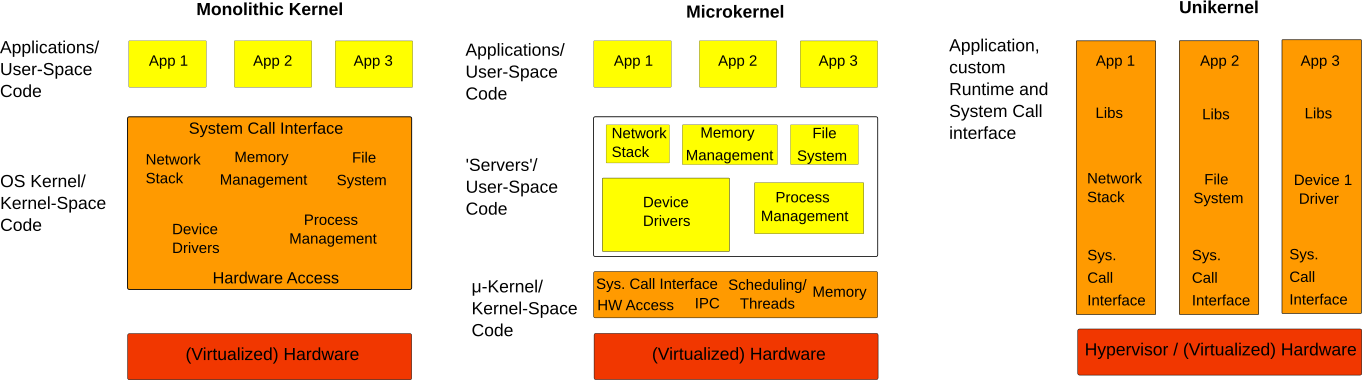
\includegraphics[scale= 0.36]{figures/kernels.png}
    \caption{Structural comparison of Monolithic, Micro- and Unikernels }
    \label{fig:kernels}
\end{figure}

\textbf{Microkernel$\blacktriangleright$} Microkernels follow a \textit{minimality principle} formulated by Liedtke~\cite{jochen1995mu} as \\

\emph{''More precisely, a concept is tolerated inside the $\mu$-kernel only if moving it outside the kernel, i.e. permitting competing implementations, would prevent the implementation of the system's required functionality.''}\\

The central motivation for microkernels, is the reduction of privileged, low-level code executing in kernel mode. Based on the insight, that large code bases of monolithic kernels com e at the costs of large potential for bugs in privileged, low-level (and therefore hard to check) code concepts to minimize kernels and therefore attack surface date back to the 70$^th$ \cite{hansen1970nucleus}. Concepts like the Mach kernel \cite{accetta1986mach}, separation kernels\cite{rushby1981design} or isolation kernels \cite{whitaker2002scale} where developed to minimize and isolate kernel space code, to increase security and enable verification.  

The minimality principle basically limits the essential components of kernel to memory management (i.e. providing access and access control to address spaces), CPU allocation (i.e. providing access to the CPU in any form of process or thread abstraction and scheduling) and inter-process communication (IPC). Other services as I/O, device drivers, networking and others run as userland processes although there might be further distinctions from actual user processes. In addition to the advantage of the smaller attack surface, the low memory requirement also makes microkernels advantageous, especially for embedded systems. 

This design comes with an inherent performance penalty. In a monolithic system a userspace application requiring access to hardware or system services would cause a single context switch to kernel mode. The request would be answered and the result returned to the userspace process. In a microkernel on the other hand, the request of the user application will be forwarded by the kernel via IPC e.g. to a driver process, who again answers via IPC indirected through the kernel. In this simple scenario the number of context switches doubles from two to four. Also the communication among system services is just function calls in monoliths while it again involves IPC and four context switches for each invocation among services. 

Currently existing examples of microkernels are L4 (formerly L3 \cite{liedtke1993persistent}), Minix \cite{herder2006minix}, Singularity \cite{hunt2005overview} or the QNX microkernel OS\cite{hildebrand1992architectural} used in embedded systems for example in phones, or as real time OSs in cars.

\textbf{Unikernels\cite{madhavapeddy2014unikernels} $\blacktriangleright$}: Unikernels also tackle the problem of large code base and attack surface in monolithic kernels. However they follow another approach concerning process isolation. The 'uni' in unikernels refers to the idea of compiling a specific kernel for each application or even component of larger applications. Basis for compilation is a library operating system written in rather high level languages, the user program and a configuration file to specify the target architecture and the required library components. Library operating systems provide functionalities of monolithic kernels as independent library implementations, for example device drivers for physical NICs are implemented in libraries that can be combined with potentially different implementations of the TCP/IP stack. Examples of library operating systems are  MirageOS\cite{madhavapeddy2013unikernels}, Graphene~\cite{tsai2014Graphene}, IncludeOS~\cite{bratterud2015includeos} or Unikraft~\cite{kuenzer2021unikraft}.
In the compiled unikernel, all processes run with kernel privileges and have direct access to the hardware or hardware abstraction layer (e.g. a hypervisor). This reduces size and attack surface compared to monolith and has unlike monolith and microkernels also no IPC overhead for context switches. 
It is not well suited, and not intended to be used for multi-user scenarios. However large applications can be realized with unikernels by distributing the app components into several distinct unikernels. In cloud applications this setup allows the hypervisor to scale only required parts of the application. 

\todo[inline]{What kind of organization is unikernel.org? \cite{unikernelorg}}
Examples of this are CubicleOS~\cite{sartakov2021cubicleos}, FlexOS~\cite{lefeuvre2021flexos} and M$^3$x~\cite{Asmussen:M3x}, M$^3$v~\cite{Asmussen:M3v}.
\todo[inline]{read \cite{madhavapeddy2014unikernels},CubicleOS~\cite{sartakov2021cubicleos}, FlexOS~\cite{lefeuvre2021flexos} and M$^3$x~\cite{Asmussen:M3x}, M$^3$v~\cite{Asmussen:M3v} \means how are the kernels compiled, what's there scope? }


\section{The M\textsuperscript{3} Operating System}
\subsection{The Concept}
M$^3$\cite{Asmussen:M3x} is a microkernel concept/architecture for distributed and potentially heterogeneous architecture, as for example different embedded processors cooperating in modern cars. It comprises a hardware and a corresponding software, i.e. OS and kernel design. Specifically the hardware design describes the components necessary to connect and control separate chips e.g. for broadband communication, signal processing (camera, GPS), or cryptographic operations, while the corresponding operating system provides communication and access to the hardware for the apps running on each component.

An overview of the principle design of M$^3$ is shown in Figure~\ref{fig:m3}. The architecture is composed of tiles, communicating with each other via data transfer units (DTU). There is only one tile, that runs the actual microkernel. This tile is also the only one requiring a general purpose core (GPC) as underlying hardware. The computing units (CU) inside the other tiles might be general purpose CPUs, FPGAs, DSPs or fixed-function accelerators. Processes on CUs run independently and isolated from each other. They can however communicate to each other via the DTUs.

The kernel is responsible for scheduling tasks on the CUs. Running tasks are called activities. On tiles using CPUs, an activity is basically a running system thread. Via the DTUs, the kernel can also control context switches between activities on the CUs and establishing communication relations between activities. By default, activities run in their own address space and are disconnected from each other. To establish a connection an activity \code{A} would once request the kernel to connect, for instance to an activity \code{B} running the network stack. Once that connection is established, the activities can directly communicate without involving the kernel again which eliminates some of the communication overhead in other microkernel systems. 

\begin{figure}[H]
    \centering
    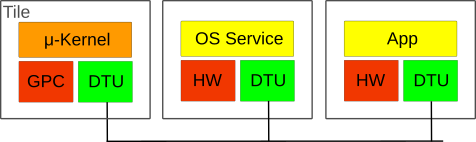
\includegraphics[scale= 0.7]{figures/m3.png}
    \caption{The m3 architecture is composed of tiles, communicating via data transfer units (DTU)}
    \label{fig:m3}
\end{figure}

In Section~\ref{subsec:BackendRequirements} we discussed the assumptions Ohua makes about backend architectures' tasks and channels. In particular we noticed, that tasks have to be cooperatively scheduled and channels have to ensure in-order, guaranteed delivery. So we take a look on if this requirements are fulfilled by M$^33$.
When activities idle they notify the kernel, which can then schedule another activity. So cooperative scheduling is given. Communication channels are unidirectional, first-in-first-out connections. Activities are not aware if their communication partner is currently running or suspended i.e. context was switched by kernel. The hardware (i.e. the DTU of the receiving tile) detects attempts to communicate with a not-running activity and errors back to the sending activity. Upon such error, the sending activity invokes the kernel to schedule the required receiving activity. The kernel buffers messages for the receiver in this case. Despite this fallback mechanism, the authors state that message delivery has only-once semantic, so data-access can/must be repeated if necessary upon failure. So we will need discuss the issue of potential message loss later in this work. 
\todo[inline]{I don't like the last sentence, but that's probably the only thing we learn from it right now}

\subsection{The Rust API}
M3 provides a Rust integration to access its abstractions of processes and channels. We will now briefly describe the main features of this API. \\

A simple example of how an activity can be instantiated is shown in Figure~\ref{fig:startingActivity}\footnote{Example adapted from \href{https://github.com/Barkhausen-Institut/M3/blob/master/src/apps/rustunittests/src/tactivity.rs}{M3 Rust unit tests}} . Activities can be initiated either on a common tile or on several tiles. In the example, the tile of the parent process is used. The API uses a closure syntax to define activities. However those definitions have no closure semantic, i.e. they do not enclose definitions from the surrounding scope.\\

To pass capabilities and file descriptors to a child activity, the attribute \rust{activity.data_sink()} can be used to serialize data into the process memory. This data can be accessed from inside the activity code using \rust{data_source()}. Serialization is implemented in a custom \rust{Serializer} based on the \rust{serde} crate. We need this mechanism, as shown in the example to pass send and receive gates to the activities. For simple environmental variables, the API provides a separate mechanism using \rust{m3::env}. This basically provides a global key-value store where variables can be stored before the definition of an activity, retrieved by key inside the activity and be deleted after the activity definition to not pollute the namespace.


\begin{figure}
    \centering
    \begin{minted}[fontsize=\footnotesize]{rust}
fn run_send_receive(t: &mut dyn WvTester) {
    // Get a descriptor of the current tile
    let tile = Tile::get("clone|own");
    // Initialize a new activity on the current tile
    let mut activity = ChildActivity::new_with(tile, ActivityArgs::new("test"));

    // initialize send and receive gate with message order, size and credits 
    let rgate = RecvGate::new(math::next_log2(256), math::next_log2(256));
    let sgate = SendGate::new_with(SGateArgs::new(&rgate).credits(1));

    // make receive gate avaible in the activities namespace
    activity.delegate_obj(rgate.sel());
    let mut dst = activity.data_sink();
    dst.push(rgate.sel();

    // define activity 
    let activity = activity.run(|| {
        ...
        // make receive gate available inside activity
        let mut src = Activity::own().data_source();
        let rg_sel: Selector = src.pop().unwrap();
        let rgate = RecvGate::new_bind(rg_sel);

        // receive 
        let mut res = recv_msg(&rgate));
        let i1 = res.pop::<u32>();
        let i2 = res.pop::<u32>();
    });

    send_vmsg!(&sgate, RecvGate::def(), 42, 23));
}
    
    \end{minted}
    \caption{Example of creating and running a Rust activity on M3}
    \label{fig:startingActivity}
\end{figure}

Concerning process communication, the API provides different mechanisms, mainly depending on the size of data to be transmitted, of which direct sending over channels is the most relevant to us. M3 manages communication among processes using capabilities. The capability to directly send to or receive from another process is implemented as \rust{Gate}s in the M3 Rust API. Gates are synchronous, directed one-to-one connections, so there are send gates \rust{SGate} and receive gates \rust{RGate}. Receive gates are instantiated with a maximum message size and a maximum overall size of the message buffer to prevent memory overflows in limited environments. The absolute (system immanent) maximum message size is 2 kb. Send gates are instantiated with a number of credits. With each message send, one credit is used. The receiver can return those credits by answering on a received message. Note that this mechanism is hidden inside the \rust{recv_msg} and \rust{send_vmsg!} calls. Both are or contain macro calls to generate and receive responses upon message receipt to pass back sending credits. \\

Apart from the credit system sending messages is straight forward as known from most pipe like interfaces. Receiving is done in two steps. First a receive stream is requested using \rust{let stream = rgate.recv_msg()}. This is a blocking call, that will return upon available messages arriving at the gate. The second step is calling \rust{let msg = stream.pop()} which is non blocking. This call can be done arbitrarily often on an existing stream but will fail if there are no more messages in the stream.\\

Finally a limitation of the current M3 API is that the standard library is not supported. There is a separate implementation of \rust{std} with essential functions but partly different function signatures. For smoltcp itself this limitation is not relevant, since it is written without using the standard library. In contrast, the libc API is a necessary part of smoltcp and is supported by M3. 

\subsection{Existing M3 Architecture Integration}
Ohua already features an architecture integration for Rust on M3. It is build on a simplified API of M3 that provides two main encapsulations, the \rust{channel()} call and the \rust{activity!} macro. Figure~\ref{fig:OhuaM3Wrapper} shows how an activity can be created using those functionalities. The function \rust{channel} basically wraps the initialization of pairs of send and receive gates with default message orderings a default message size and a default of one send credit. This allows to create channels basically the same way as in pure Rust or Python. The \rust{activity!} generates code to 1) instantiate a \rust{ChildActivity} on the current tile  2) delegate the given gates to the activity and 3) bind and activate the gates inside the activity. This again basically resembles the initialization of a thread in pure Rust. 


\begin{figure}
    \centering
    \begin{minted}[fontsize=\footnotesize]{rust}
use funs::hello_world;

fn test() -> String {
   use m3::com::channel::{Sender, Receiver};
   use m3::activity;
   let (a_0_0_tx, mut a_0_0_rx) = channel(); 
    activity!(
        (|a_0_0_child_tx: Sender| {    
            let a_0_0 = hello_world();
            a_0_0_child_tx.send(a_0_0)?;
            Ok(())
          }
        )(a_0_0_tx)
    );
    a_0_0_rx.activate()?;
    a_0_0_rx
    .recv::<String,>()
    .expect("Error message")
}

    \end{minted}
    \caption{Example of creating an activity using the simplified M3 Rust API}
    \label{fig:OhuaM3Wrapper}
\end{figure}

However, as previously explained, activities in M3 are not closures. This means that in order to use environment variables, an additional mechanism will be necessary. This is currently not yet part of the architecture integration.



\section{smolTCP}
smolTCP~\cite{smolTCP} is a Rust-based open-source implementation of a TCP/IP stack. It runs entirely as a user space application. It also provides conditional compilation features to build applications without heap allocation. This makes smoltcp and applications build with it amenable be used in microkernels as M$^3$\cite{Asmussen:M3v} and embedded systems such as ARTIQ (e.g. \cite{lam2021combining}). In fact the microkernel operating system Redox\cite{redoxwebsite}, as well as M3 itself already use smoltcp for their network stack implementation. So in both systems, smoltcp is used to create a network stack as a sequential, userspace service. This means that, in contrast to the application to be developed in this thesis, the TCP/IP layer, the actual network layer or system interface and the user application communicate with each other via shared memory. \\

The design of the library is structured according to typical TCP/IP layering. We will briefly introduce the three main layers, or components respectively, that are relevant in this work\footnote{For more information see the documentation at \url{https://docs.rs/smoltcp/latest/smoltcp/}}.


The \rust{socket} module provides different socket abstractions implementing the TCP, UDP, IGMP or DHCP protocols respectively as well as for raw sockets. Common features of all those abstractions are keeping track of inbound and outbound data in socket buffers and implementing functionality to package or unpack those data according to the implemented protocol. The sockets keep also track of additional state information, relevant for their respective protocol e.g. TCP or DHCP client states, hop limits, window sizes etc..\\

The \rust{iface} module provides the abstractions of the Ip layer. The most important structure is \rust{ Interface}. In an inner component of the interface (\rust{InterfaceInner}) the state data of the IP layer are stored. This includes the IP address of the interface, a routing table, a neighbor cache and the hardware address (depending on the transport medium according to Ethernet or IEEE 802.15.4 standard). Accordingly, the generation and interpretation of IP headers for outgoing and incoming packets are also tasks of the 
\rust{InterfaceInner}. In the currently official variant of smoltcp, the Interface also contains a field \rust{Device}, holding an abstraction of the physical network layer, and a \rust{SocketSet} to manage all sockets belonging to the interface. Smoltcp is under ongoing development and so in the recent implementation state, \rust{Device} and \rust{Sockets} are no longer part of the interface, but independent structures passed to it to process packets from sockets to device and vice-versa. We will discuss the implication of this in further detail in the Section~\ref{sec:ImplSmoltcp}. \\

Finally the physical layer is implemented in the \rust{phy} module. It provides different implementations of the \rust{Device} trait, to connect the application to the underlying operating systems loopback or tuntap interface or raw sockets. Implementors of the \rust{Device} trait provide the methods \rust{receive}, \rust{transmit} and \rust{capabilities}.\\

The actual transfer of packets from the interface to the device is realized via sending and receiving tokens. We explain in a little more detail here, because it exemplifies a characteristic of the smoltcp code. A successful call to \rust{device.receive()} will yield a tuple of a receive toke \rust{RxToken} and a send token \rust{TxToken}. The former will contain the actual received content as a private field, the later contains a reference to the device specific storage for outgoing packets. In case of tuntap and rawsocket devices, this reference is a file pointer provided by the operating system. In Figure~\ref{fig:TokensAndClosures} the implementation of a sending \rust{TxToken} for raw sockets and the usage of such token to send an Ethernet frame are shown. Two things become apparent. First, the memory for the packets is allocated only at device level upon consuming a token. Second, any structs needed to construct the frame are instantiated in a closure passed as an argument to \rust{tx_token.consume()}. As closures are realized via fixed size structs on the stack frame of the called function, this technique enables smoltcp to work without heap allocation and is used heavily in the code. This principle is used in a cascading manner i.e. \rust{dispatch_ethernet} itself also receives a closure capturing objects from the calling scope.\\

Obviously one implication of separating the layers of smoltcp to different, memory separated components is, that this kind of memory efficiency can not be maintained. 
\todo[inline]{Check and augment link to implementation/discussion section when available}

\begin{figure}[H]
\centering
\tabskip=0pt
\valign{#\cr
    \hbox{%
    \begin{subfigure}{.37\textwidth}
    \centering
     \begin{minted}[fontsize=\tiny]{rust}
// Sending Token for RawSocket

pub struct TxToken {
    lower: Rc<RefCell<sys::RawSocketDesc>>,
}

impl phy::TxToken for TxToken {
    fn consume<R, F>(
    self, 
    ..., 
    f: F) -> Result<R>
    where
        F: FnOnce(&mut [u8]) -> Result<R>,
    {
        let mut lower = self.lower.borrow_mut();
        let mut buffer = vec![0; len];
        let result = f(&mut buffer);
        match lower.send(&buffer[..]) {
            Ok(_) => result,
            // Error handling 
        }
    }
}
     \end{minted}
    \end{subfigure}%
  }
  \cr
  \noalign{\hfill}
    \hbox{%
    \begin{subfigure}{.62\textwidth}
    \centering
    \begin{minted}[fontsize=\tiny]{rust}
    //Interface using a TxToken to send a frame
    
    pub fn dispatch_ethernet<Tx, F>(
    &mut self, 
    tx_token: Tx, 
    buffer_len: usize, 
    f: F) -> Result<()>
    where
        Tx: TxToken,
        F: FnOnce(EthernetFrame<&mut [u8]>),
    {
        let tx_len = EthernetFrame::<&[u8]>::buffer_len(buffer_len);
        tx_token.consume(self.now, tx_len, |tx_buffer| {
            ...
            let mut frame = EthernetFrame::new_unchecked(tx_buffer);
            let src_addr = {...};
            
            // closure from outer scope:
            f(frame);
            Ok(())
        })
    }
    \end{minted}
    \end{subfigure}%
  }
  \vfill
  \cr
}
\caption{Sending and receiving packages is implemented via Tokens exposing a \rust{consume} method, taking closures as argument that process the send or received content. This way, memory allocation can be constrained a) to the device layer and b) to the stack if necessary}
\label{fig:TokensAndClosures}
\end{figure}



\section{Rust}
\label{subsec:Rust}
The main questions of this thesis are i) What requirements must a sequential program meet in order to be converted into a concurrent program in a semantics-preserving way? and ii) What steps are necessary for the conversion? Rust as a programming language is particularly well suited to investigate these questions. This is due to Rusts extended type system, that can not only enforce well-typedness of a program but also statically ensure the validity of references and therefor safety of memory usage at runtime. The two central concepts enabling this are \emph{ownership} and \emph{lifetimes}.\\

\emph{Ownership} is used to ensure memory safety in (safe) Rust. In particular, it allows the Rust compiler to ensure at compile time that no two pieces of code can modify an object at any time, i.e. that at runtime there is never more than one reference to an object that allows write access. 

\emph{Lifetimes} extend the concept of ownership to track the validity of references. This model prevents not only frequent errors in sequential programs, it enforces also already a substantial part of the assumptions of a distributed programming model. Therefore necessary restrictions of a distributed, concurrent programming model are particularly well to be examined in Rust, because they are already enforced in the sequential code. 

In Chapter~\ref{Chapter:Implementation}, we will refer to those concepts and their implications for our findings. So to better understand these implications, we will first take a closer look at the rules of ownership and lifetimes here.

\textbf{Ownership:}
Rust has neither garbage collection, nor does the user need to free and allocate memory herself. Instead Rusts runtime manages memory using ownership and lifetime rules. The Rust compiler ensures, for most types statically, that there is exactly one \emph{owner} of each value i.e. one variable holding it, created either on heap or stack. When this owner goes out of scope, the value is cleared from memory without the need for extensive reference tracking garbage collection.
This is realized by automatic implementations of the \rust{drop} function for every type. A call to \rust{drop} is added automatically by the compiler for each variable as it goes out of scope i.e. when the scope it has been declared in ends.

Ownership has a different implementation for values located on the stack and on the heap. For values stored on the stack, the owner is simply the variable assigned to that value. For a value allocated on the heap, the variable owning that value holds a pointer to the memory location of that value and additional information as for instance actual and totally allocated size of the value. This difference is important for the semantics of passing values as function arguments or returning them from functions. The act of passing values directly i.e. not only passing a reference is called \emph{moving} in Rust parlance. For both the stack based and the heap based values, \emph{moving} means copying the owner, i.e. copying the information the owner holds on the stack, to the stack frame of the called function. Returning values also follows that principle. But as we noticed before, for stack based values this actually also copies the value itself. This results in a new value, with a new owner and allows the old owner to remain valid. For heap based values on the other hand, only the memory reference to the value is copied that way. So to prevent having several owners addressing the same memory location, the old owner gets invalidated upon \emph{moving}. To actually duplicate heap data, one needs to implement or derive the \rust{Clone} trait for the data type. An explicit call to the \rust{clone()} method will then deepcopy the heap allocated data and its owner, resembling the semantics of implicit copy on stack based values.

In a distributed scenario, passing a value to a function call will involve transferring that value to another processes memory that we do not expect to sync with the original location. So, like it is enforced by the Rust compiler we can not use the original reference to that value any more, since it would lead to inconsistent states. In fact Ohuas programming model, at least theoretically is more strict than that of Rust. While it always assumes pure function arguments to be used immutably i.e. read-only, it also currently requires variables to be used only once. 
\todo[inline]{Check with Sebastian:}
\question{Ohua programming model says, we expect arguments of functions (other than the self argument) to be read-only. Why should we then further restrict the programming to make variable use linear instead of assuming copy?}

\textbf{References:} Obviously, besides passing the value directly, Rust also offers the possibility of creating references to both stack and heap based values. In contrast to pointers, Rusts references are guaranteed to address valid data. References do not convey ownership. In Rusts memory model this means, references are just an address to the owner, and do not contain information like the size and capacity of the data pointed to. Passing values by reference is called \emph{borrowing} in Rust terminology. References just as  values are immutable by default. The general rule for borrowing a value is, that at each point in the code there can only be either one mutable, or an arbitrary number of immutable references to each owner. References are values themselves i.e. they have an owner and a lifetime tied to the scope they are valid in. So Rust can track validity of reference owners to enforce the borrowing rules. Beyond scope validity the rust compiler is capable of identifying the last use of a reference and shorten its lifetime to this point (a concept called 'non-lexical lifetimes'). Therefore it is possible to borrow a value mutably multiple times within a scope. When one mutable reference is created and used only after the last use of another one, the compiler can shorten the former ones lifetime to end before the next reference becomes valid. 

\textbf{Lifetimes}\footnote{ We will focus on the main aspects for this work here, but a full introduction to Lifetimes, as well as rules for subtyping and inference can be found in the Rust Book\cite{rustbook} and the Rust Reference\cite{rustreference} in the Chapter \emph{Subtyping and Variance}.}: As explained before, references do not convey ownership. So \emph{lifetimes} are Rusts way to ensure, that the owner a reference is pointing to is not dropped while the reference is still in use. 
In general every reference has a lifetime. Inside a single function scope, lifetimes are mostly implicit. The compiler can simply derive them from the local scoping. However when references are used as an argument or return value lifetimes can not in general be derived by the compiler and need to be made explicit. Note that the constructors of \rust{enum} and \rust{struct} types are essentially also just functions, taking fields as arguments and returning the respective \rust{emun} or \rust{struct}. So obviously they also have to abide lifetime rules. 

As we noticed, lifetimes are meant to ensure reference validity. The mechanism is best explained using the case of function return values. Returning valid values, either by value or by reference from a function is only possible, if the owner of that value will not be dropped at the end of the function. This is the case if 
\begin{enumerate}[a)]
    \item The function returns a moved owner: The returned value is allocated on the heap and the actual owner is returned. This will result in a move, copying the owners reference information to the return stack frame
    \item The functions returns a copied owner: The returned value is allocated on the stack, but implements \rust{Copy}. This will copy the value itself to the return stack frame
    \item The function returns a reference to the owner: The actual owner of the value lives in the outer scope and is manipulated by reference in the function. If a reference to the original owner is returned, the owner will continue to be mutably borrowed for the lifetime of this reference. This also includes references to static memory, e.g. string literals known at compile time. 
\end{enumerate}

When are lifetime annotations needed?: The simple answer is, whenever there are references and the compiler can not infer them automatically. The first two cases generally do not require lifetime annotations. In case a) the data lives on the heap, but the 'owning information' is copied to the return scope so Rustc can automatically infer its lifetime further on by tracking the owner. In case b) the data is copied to the stack of the return scope and again the compiler can automatically infer scopes and lifetimes. In case c) however the lifetime of the reference returned is bound to the lifetime of the memory location (reference) passed as a parameter. The reason why not every function accepting and/or returning references needs lifetime annotations in parameters, return value and the function itself is so called 'lifetime elision'. Rust uses a set of rules to automatically annotate lifetimes in standard situations, which are
\begin{enumerate}
    \item In a function declaration \rust{fn fun(a:&A, b:&B, ...)-> &Z} all references are assigned a freshly generated lifetime parameter \rust{fn fun<'a, 'b, ..., 'z>(a:&'a A, b:&'b B, ...) -> &'z Z}
    \item If there is only one input reference \rust{fn fun<'a>(a:&'a A) -> &'a Z}, its lifetime is also assigned to the output reference
    \item If the function is a method \rust{fn fun<'self, 'a, ... >(& 'self self, a:&'a A,...) -> (&'self Z1, &'self Z2} all outputs are assigned the lifetime of the object acted on.
\end{enumerate}

The same lifetime rules that hold for function arguments and returns basically hold for structs. A \rust{struct} holding a reference in a field, requires that reference to come from a surrounding scope. Just as a function can not take a reference that might not live as long as the function runs, a \rust{struct} can only live as long as the shortest living reference it holds. The same holds for \rust{enum}s obviously. Just like for functions this means, those \rust{struct}s and \rust{enum}s are generic over at least one lifetime parameter, determined by the reference they are given on creation.

When those rules are insufficient, annotations are needed. For example if there are multiple input references and a specific one should provide the lifetime information for the output. Also automatic inference might lead to unwanted effects. For instance if a reference to a \rust{static} value is passed to a function, the compiler will infer the returned reference to also live for \rust{static}. This means the original value can not be borrowed mutably or even immutable again in the program. In this case lifetime annotations help the compiler to solve lifetime unification at all or in a more favorable way. \\

So when and why would we need to consider lifetimes? We expect the programmer to provide valid input Code to the compilation. Also the programming model of Ohua prohibits reference arguments in scope. So up to this point, there was no necessity to consider lifetime implications in the transformations Ohua applies to the code. However in this work, we will not only manipulate the code 'in scope' but also inside the components that will later be opaque to Ohua. It is possible, and for efficiency reasons desirable to keep on working with references inside those components. Meanwhile we will also introduce and in particular split existing functions. Therefore we will need to consider constraints and effects of reference lifetimes on our transformations.




